\section{Laser power control}

This section discusses the concepts behind laser power stabilization, as well as
the performance of the system tested using the laser power control PCB. See
Fig.~\ref{AOM_idea} for a diagram of the control system.

\subsection{Basic control theory}

In order to evaluate the performance of the power stabilization system, it is
helpful to learn some basic principles of control theory. In this section, I
define different types of control, bandwidth in analog and digital systems.

In general, there are two broad types of control systems, either open loop or
closed loop (Fig.~\ref{control_types}). Consider a linear, frequency-dependent
amplifier, where the inputs and outputs are given by
%
\begin{align*}
   V_\text{in}&=V_0\sin(\omega t)\\
   V_\text{out}&=A(\omega)V_0\sin(\omega t+\phi(\omega)).
\end{align*}
%
For this open-loop control system, the behavior is determined by the
\emph{open-loop gain} $A(\omega)$ and the phase shift $\phi(\omega)$. Thus we
can control the output if we know $A(\omega)$ and $\phi(\omega)$, i.e.,
calculate the required input to produce a certain output.

\begin{figure}
   \centering
  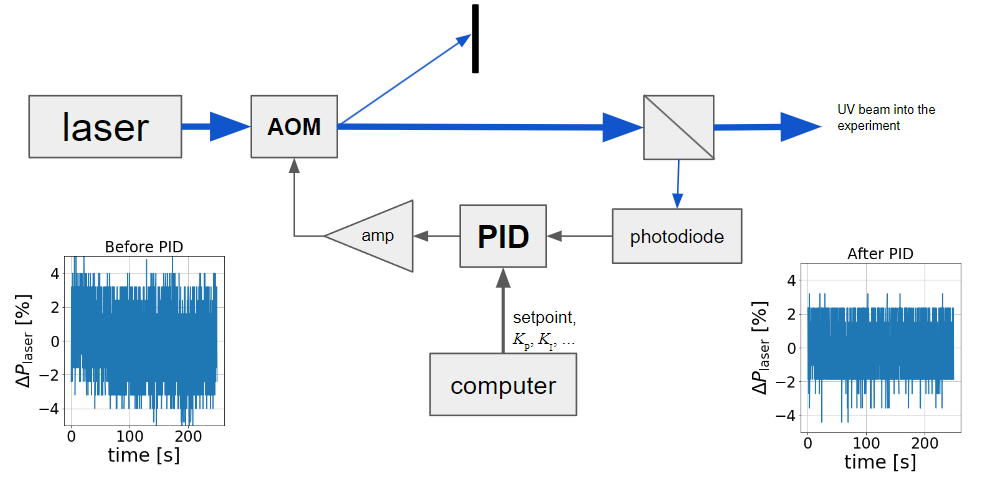
\includegraphics[width=\textwidth]{figs/todo/AOM_idea.png}
   \caption{Signal path for laser power stabilization.}
  \label{AOM_idea}
\end{figure}

\begin{figure}
   \centering
  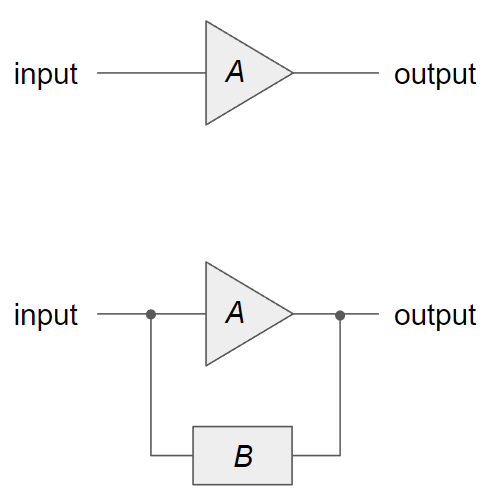
\includegraphics[width=.49\textwidth]{figs/todo/control_types.png}
  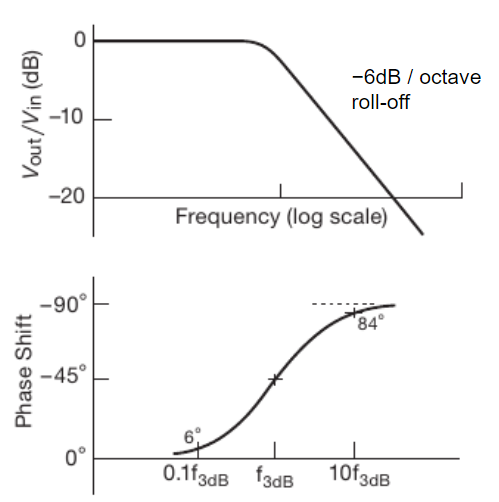
\includegraphics[width=.49\textwidth]{figs/todo/bode.png}
   \caption[Open vs closed loop control; Bode plot.]{\part{Left} Open loop vs
   closed loop control. \part{Right} Bode plot of gain and phase versus
   frequency. Figure adapted from \cite[Fig.~4.97]{horowitz2016art}}
  \label{control_types}
\end{figure}

As an example, consider the plot of gain and phase versus frequency for a simple
single-stage $RC$ filter section (Fig.~\ref{control_types}). The output at a
constant input amplitude drops proportionally with the input frequency, i.e.\
the output voltage drops by a factor of 2 when the frequency doubles (a.k.a.,
increases by an octave). Thus the `power' decreases by a factor of 4, which can
also be represented in units of decibel as $10\log_{10}4\approx6.02$, hence the
$-6$~dB/octave roll-off noted on the figure. At the same time, as the frequency
passes the `corner frequency' $f_\text{3~dB}$, there is a 90-degree phase shift.

The open-loop gain for an opamp looks very similar. Consider the example in
Fig.~\ref{opamp} and note the similarity with an $RC$ filter. In fact, the gain
roll-off is intentionally added to the amplifier to decrease gain at high
frequencies for stability purposes. The plot of the open-loop gain demonstrates
the large gain characteristic of opamps (100~dB corresponds to a voltage gain of
$10^5$). It also suggests two ways of quoting the bandwidth of the amplifier. We
can either give the bandwidth over which the open-loop gain is relatively flat;
in the example shown, that is approx.\ 10~Hz. The more common number is the
so-called gain--bandwidth product or GBP (approx.\ 1~MHz), which can be read off
as the frequency at which the gain falls to unity. (In general, the GBP could be
different at different gains, but opamps are typically designed with a simple
one-pole roll-off, such that the GBP is independent of gain and can be most
easily found by looking at unity gain.)

\begin{figure}
   \centering
  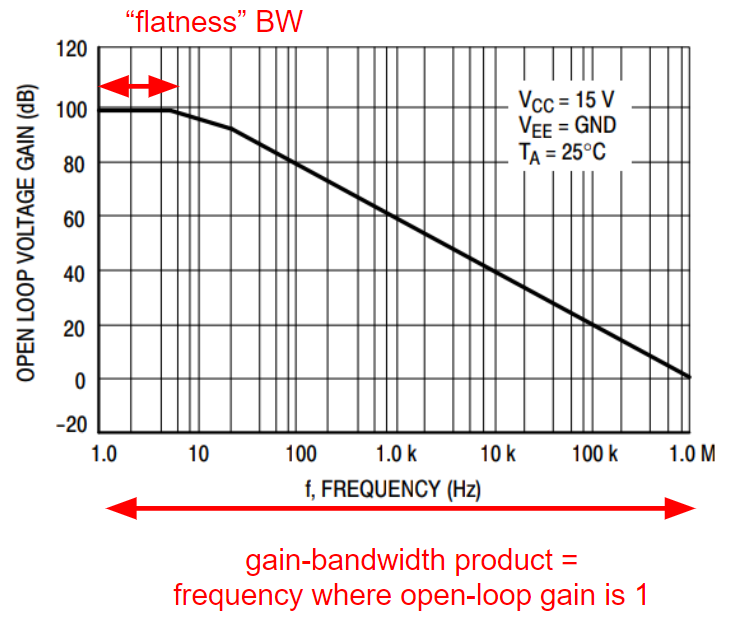
\includegraphics[width=.49\textwidth]{figs/todo/opamp.png}
  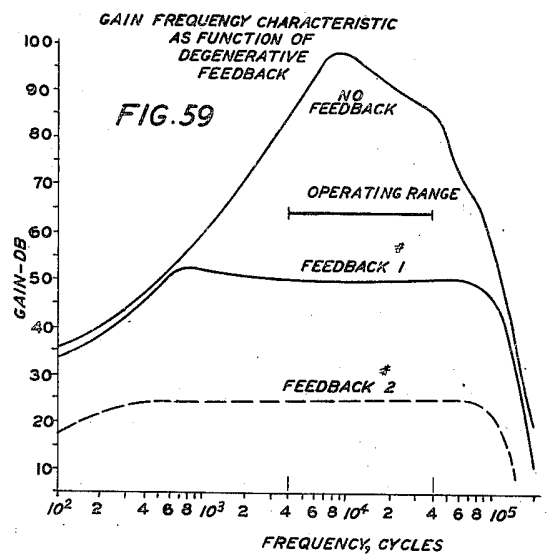
\includegraphics[width=.49\textwidth]{figs/todo/feedback.png}
   \caption[Open and closed loop gain vs frequency.]{\part{Left} Open loop gain
   vs frequency. Adapted from a LM324 datasheet. \part{Right} Bandwidth vs
   frequency, from \cite{black1935wave} as quoted in
   \cite[Fig.~2.87]{horowitz2016art}.}
  \label{opamp}
\end{figure}

We have seen that the frequency range over which the open-loop gain of an opamp
is flat is often surprisingly low (10~Hz in the case of LM324). However, there
is a way to trade off the magnitude of the gain for an increase `flatness'
bandwidth: closed-loop control. As show in Fig.~\ref{control_types}, an inverted
fraction $-B$ of the output is fed back into the input of the amplifier $A$.
This of course decreases the output magnitude:
%
\[
   V_\text{out}=A(\omega)\left[V_\text{in}-B(\omega)V_\text{out}\right]
   \quad\to\quad
   V_\text{out}=\frac{A}{1+AB}V_\text{in}.
\]
%
In the limit of large $A$, this becomes
%
\[
   \lim_{A\to\infty}V_\text{out}=\frac{1}{B}V_\text{in}.
\]
%
Thus, the frequency dependence of the open-loop gain $A(\omega)$ drops out of
the equation and the overall gain (the closed-loop gain) of the system is almost
entirely determined by the frequency response of the feedback network $B$. The
latter can usually be arranged to have an essentially flat frequency response.
Of course, this only works at frequencies at which $A$ is sufficiently large.
See Fig.~\ref{opamp} (right side) for an illustration of how the technique of
feedback dramatically flattens out the gain vs frequency.

In the above, the open loop gain $A$ was that of an (operational) amplifier.
However, the control problem is general, and $A$ could be anything that has an
input and produces a certain output. By arranging for part of the output to be
fed back into the input, we greatly simplify the control of the output. This is
especially the case when $A$ is time-dependent or noisy. Insofar as $A$ is large
enough, we can suppress this time dependence or noise by turning up the gain $B$
of the feedback network. In the following section, I discuss how to arrange that
$A$ is large enough to make closed-loop control possible.

\subsection{Proportional and integral control}

The ideal case for a control system is that of a follower (Fig.~\ref{follower}).
When a follower is working as it should, the input is directly translated to the
output with at most a change of units. For example, if we were able to set up a
laser power control system as a follower, the input voltage (or DAC code) would
be linearly proportional to the output power, with no noise or other
time-dependence at all.

\begin{figure}
   \centering
  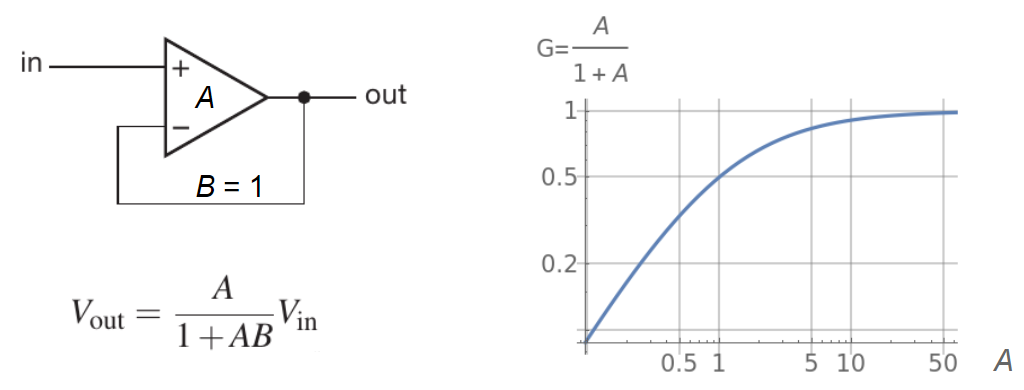
\includegraphics[width=\textwidth]{figs/todo/follower.png}
   \caption{Non-ideal voltage follower: gain is only truly unity when $A$ is
   very large.}
  \label{follower}
\end{figure}

Of course, in real life $A$ is not a simple gain block where we can almost
arbitrarily arrange a very large gain. For example, in the case of laser power
control, $A$ consists of the photodiode and its electronics, an RF amplifier and
amplitude control of the RF, the sound propagation in the AOM, as well as
possible converter in case of digital system. While it is easy to insert an
electronic amplifier in this signal chain, in practice the maximum achievable
gain is limited by the time the signal takes to travel through the signal chain.
In frequency domain, this time would be considered a phase shift, and if it is
large enough can invert the sign of the feedback. Thus instead of negative
feedback, which reduces the overall gain but increases the bandwidth, we would
have positive feedback, which causes oscillation.

A simple solution would be to turn up the gain for slow perturbations, while
keeping the higher frequencies intact. This can be done using integral control.
In time domain, the integral keeps track of the total accumulated error. The
output of an integrator is given as
%
\[
   V_\text{out}(t)=K_\text{i}\int_0^t V_\text{in}(t')\d t',
\]
%
where $K_\text{i}$ is the integral constant. In frequency domain, we see that
integral control amplifies low frequencies more than the high:
%
\[
   V_\text{out}(\omega)=K_\text{i}\frac{V_\text{in}(\omega)}{i\omega}.
\]
%
An integrator inserted in the signal chain can thus help realize a nearly-ideal
follower situation at lower frequencies, without risking instabilities at high
frequencies.

\subsection{Digital systems}

If the control system's signal chain contains a digital section, we have to
consider how this affects the performance of the control system. In this
section, we briefly review the impact of digitization on the bandwidth and
noise.

\paragraph{Bandwidth}



\paragraph{Noise}


